\documentclass{article}
\usepackage{fancyhdr}
\usepackage[utf8]{inputenc}
\usepackage[english]{babel}
\usepackage{tikz, multicol, graphicx, etoolbox, enumerate, setspace, relsize, mathrsfs, verbatim}
\usepackage{amsmath, amsfonts, amssymb, amsthm, epsfig, epstopdf, titling, url, array, esvect, tikz-3dplot}
\usepackage{graphicx}
\usepackage{hyperref}

\usepackage{listings}
\usepackage{xcolor}

\definecolor{codegreen}{rgb}{0,0.6,0}
\definecolor{codegray}{rgb}{0.5,0.5,0.5}
\definecolor{codepurple}{rgb}{0.58,0,0.82}
\definecolor{backcolour}{rgb}{0.95,0.95,0.92}

\usepackage{pgfplots}
\usepackage{tcolorbox}
\usepackage{amsthm}
\usepackage{cancel}
\usepackage[left=1in,right=1in,top=1in,bottom=1in]{geometry}
\usepackage[tableaux]{prooftrees}

\lstdefinestyle{mystyle}{
    backgroundcolor=\color{backcolour},   
    commentstyle=\color{codegreen},
    keywordstyle=\color{magenta},
    numberstyle=\tiny\color{codegray},
    stringstyle=\color{codepurple},
    basicstyle=\ttfamily\footnotesize,
    breakatwhitespace=false,         
    breaklines=true,                 
    captionpos=b,                    
    keepspaces=true,                 
    numbers=left,                    
    numbersep=5pt,                  
    showspaces=false,                
    showstringspaces=false,
    showtabs=false,                  
    tabsize=2
}

\lstset{style=mystyle}

\pagestyle{fancy}
\fancyhf{}
\fancyhead[L,RO]{Tasksheet 8}
\fancyhead[R,RO]{Fundamentals of Computational Mathematics}
\fancyfoot[L,RO]{Xiang Gao}
\fancyfoot[R,RO]{Math 4610}
\renewcommand{\headrulewidth}{0.4pt}% Default \headrulewidth is 0.4pt
\renewcommand{\footrulewidth}{0.4pt}% Default \footrulewidth is 0pt
\def\checkmark{\tikz\fill[scale=0.4](0,.35) -- (.25,0) -- (1,.7) -- (.25,.15) -- cycle;} 

\begin{document}

\section*{Task 1}
I have created the following code that implement Gaussian elimination and backsubsitution for square linear systems of equations. The code is documented \href{https://github.com/GoByMark/math4610/blob/main/Homework_Tasks/Tasksheet_08/src/Task_1.py}{here} in the \href{https://github.com/GoByMark/math4610/blob/main/Homework_Tasks/Software_Manual/Software_Manual_toc.md}{Software Manual}.\\
\lstinputlisting[language=Python]{Task_1.py}

\newpage

with the following output:
\begin{center}
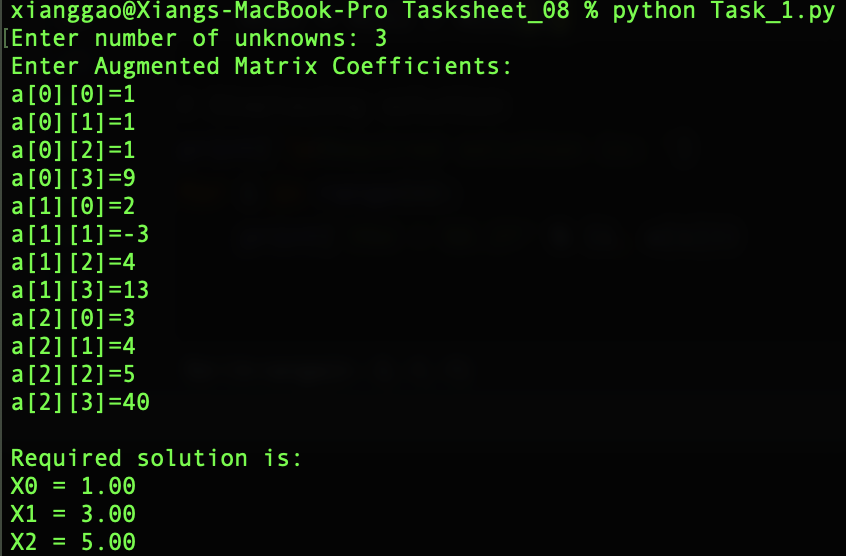
\includegraphics[width=\textwidth]{Screenshots/1.png}\\
{\bf Figure 1.} Running the Task 1.py From the Terminal.
\end{center}

\section*{Task 2}
I have created the following code that implement forward substitution. The code is documented \href{https://github.com/GoByMark/math4610/blob/main/Homework_Tasks/Tasksheet_08/src/forSub.py}{here} in the \href{https://github.com/GoByMark/math4610/blob/main/Homework_Tasks/Software_Manual/Software_Manual_toc.md}{Software Manual}.\\
\lstinputlisting[language=Python]{forSub.py}
I have also created the following code that implement LU-factorization. The code is documented \href{https://github.com/GoByMark/math4610/blob/main/Homework_Tasks/Tasksheet_08/src/Task_2.py}{here} in the \href{https://github.com/GoByMark/math4610/blob/main/Homework_Tasks/Software_Manual/Software_Manual_toc.md}{Software Manual}.\\
And the testing matrix $A$ is 
$$A = \begin{bmatrix}
7 & 3 & -1 & 2\\
3 & 8 &  1 & -4\\
-1 & 1 & 4 & -1\\
2 & -4 & -1 & 6
\end{bmatrix}$$
\lstinputlisting[language=Python]{Task_2.py}
\begin{center}
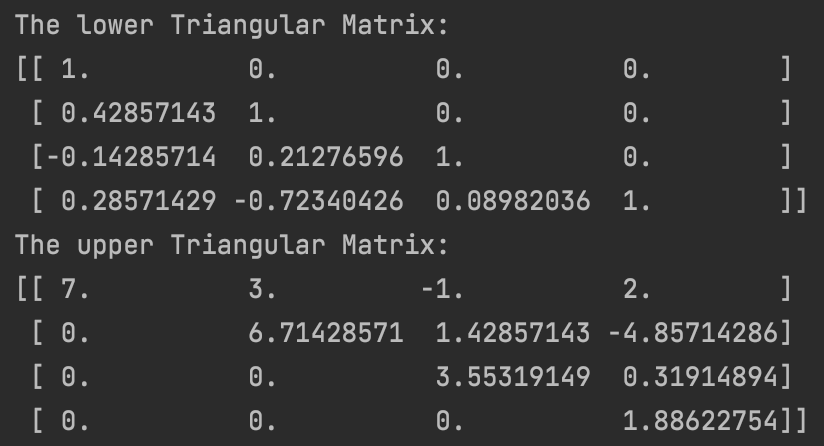
\includegraphics[width=\textwidth]{Screenshots/2.png}\\
{\bf Figure 2.} Result of Running the Task 2.py.
\end{center}

\section*{Task 3}
I have created the following code that uses LU-factorization on Hilbert matrices of size $n = 4, 5, \dots, 10$. The code is documented \href{https://github.com/GoByMark/math4610/blob/main/Homework_Tasks/Tasksheet_08/src/Task_3.py}{here} in the \href{https://github.com/GoByMark/math4610/blob/main/Homework_Tasks/Software_Manual/Software_Manual_toc.md}{Software Manual}.\\
\lstinputlisting[language=Python]{Task_3.py}

with the following output:
\begin{center}
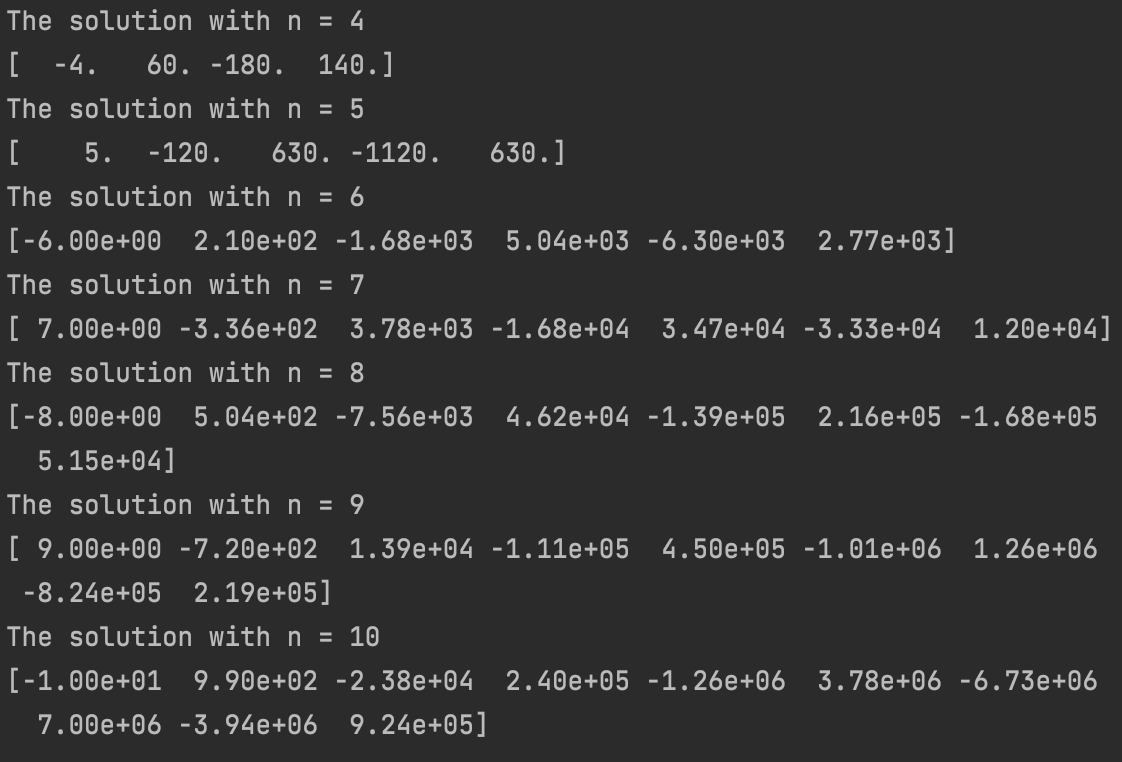
\includegraphics[scale = 0.6]{Screenshots/3.png}\\
{\bf Figure 3.} Result of Running the Task 3.py.
\end{center}

\section*{Task 4}
I have created the following code that implements scaled partial pivoting for the Gaussian elimination method for solving linear systems of equations. The code is documented \href{hhttps://github.com/GoByMark/math4610/blob/main/Homework_Tasks/Tasksheet_08/src/Task_4.py}{here} in the \href{https://github.com/GoByMark/math4610/blob/main/Homework_Tasks/Software_Manual/Software_Manual_toc.md}{Software Manual}.\\
And the testing matrix $A$ is 
$$A = \begin{bmatrix}
7 & 3 & -1 & 2\\
3 & 8 &  1 & -4\\
-1 & 1 & 4 & -1\\
2 & -4 & -1 & 6
\end{bmatrix}$$ where the vector $b$ is
$$b = \begin{bmatrix}1, 1, 1, 1\end{bmatrix}$$
\lstinputlisting[language=Python]{Task_4.py}
with the following output:
\begin{center}
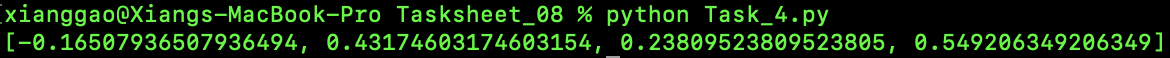
\includegraphics[width=\textwidth]{Screenshots/4.png}\\
{\bf Figure 4.} Result of Running the Task 4.py.
\end{center}

\section*{Task 5}
I have created the following code that uses LU-factorization on Hilbert matrices of size $n = 4, 5, \dots, 8$. The code is documented \href{https://github.com/GoByMark/math4610/blob/main/Homework_Tasks/Tasksheet_08/src/Task_5.py}{here} in the \href{https://github.com/GoByMark/math4610/blob/main/Homework_Tasks/Software_Manual/Software_Manual_toc.md}{Software Manual}.\\
\lstinputlisting[language=Python]{Task_5.py}
with the following output:
\begin{center}
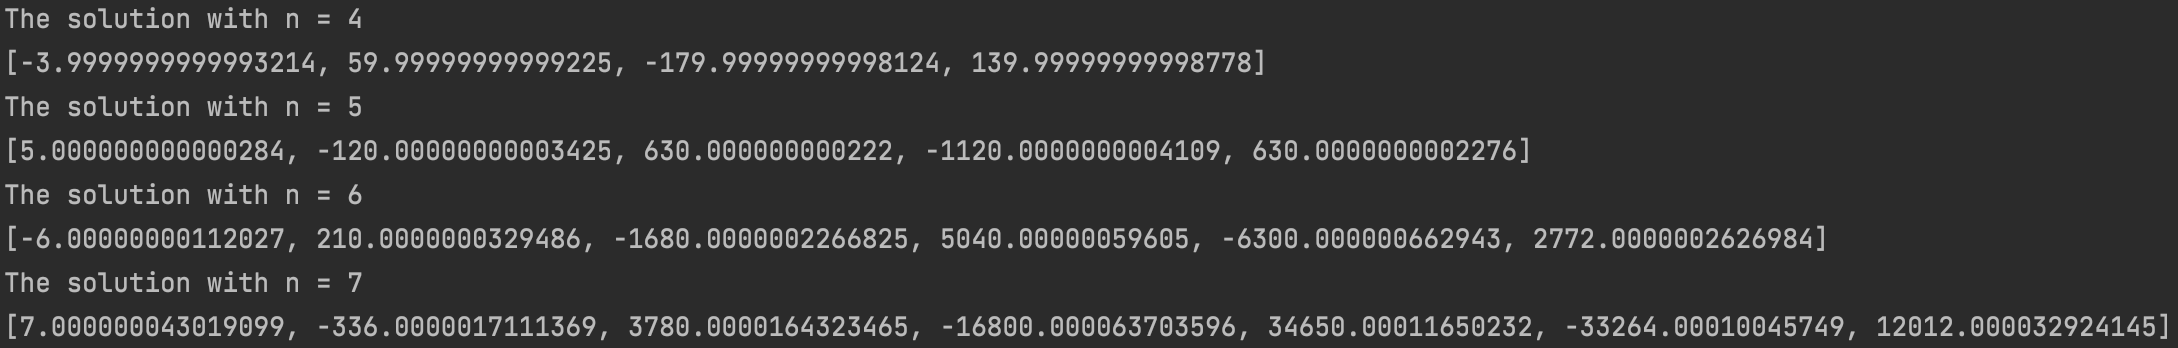
\includegraphics[width=\textwidth]{Screenshots/5.png}\\
{\bf Figure 5.} Result of Running the Task 5.py.
\end{center}


\section*{Task 6}
The Hilbert Matrix is a popular Matrix throughout Mathematics. In \href{https://www.tandfonline.com/doi/abs/10.1080/00029890.1983.11971218}{this article}\footnote{https://www.tandfonline.com/doi/abs/10.1080/00029890.1983.11971218} I found, specifically, its use in studying digital computing during its early days. The Hilbert Matrix has a condition number that grows rapidly as the square matrix grows in number of columns/rows. Below is the growth rate for the asymptotic growth rate for the 2-norm:
$$\kappa_2\left(H_n\right) \sim e^{3.5n}$$
And in \href{https://nhigham.com/2020/06/30/what-is-the-hilbert-matrix/}{this article}\footnote{https://nhigham.com/2020/06/30/what-is-the-hilbert-matrix/} I found, there exists multiple ways of generating the Hilbert Matrix that's both beneficial to Computer Scientists and Mathematicians.
\end{document}